\section{Mākoņainība Latvijā}
%Enter antagonists. Mākoņi. Bloķē daudz saules apstarojuma. Cik LV mākoņainu dienu?
%Izanalizēt VTPMML meteo datus no 2013.
%Pajautāt Stasim kļūdas.

Tiek apskatīta atmosfēras un mākoņu ietekme uz virsmas saņemto saules starojumu, un tās praktiskā nozīme, apstrādājot pieejamos Saules starojuma datus.

Kopējais mākoņu daudzums tiek iedalīts 10 klasēs no 0 (pilnīgi skaidrs) līdz 1 (pilnīgi apmācies). Mākoņainība Rīgā var sasniegt līdz 60\% jūlijā un līdz pat 90\% decembrī (skat.~\ref{fig:makoni_Riga}. att.). Tas nozīmē, ka Saules paneļu efektivitātes novērtējumam Latvijas klimatā mākoņainība ir ļoti būtiska un tā palīdzēs prognozēt nepieciešamos enerģijas uzkrājumus un papildavotus, ja solārā enerģija tiek izmantota kā pamata enerģijas avots.
\begin{figure}[h]
	\centering
	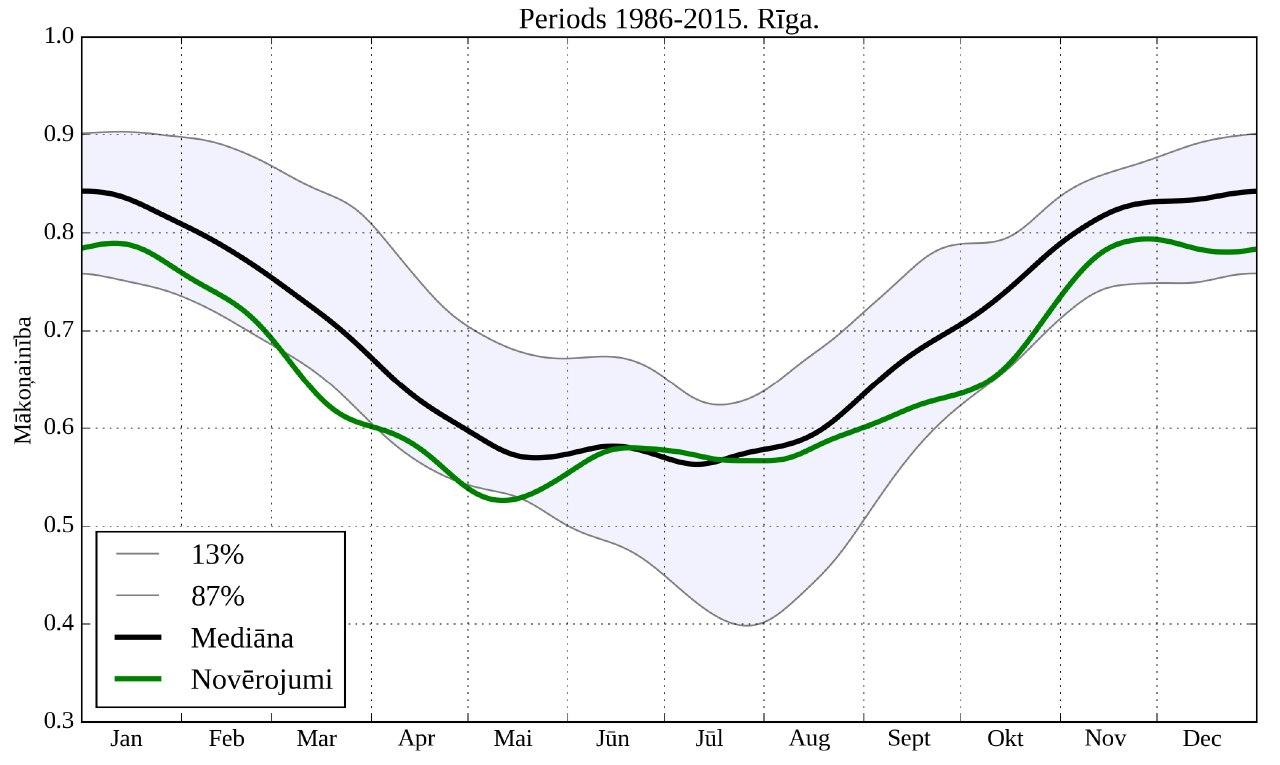
\includegraphics[width=0.8\linewidth]{figures/misc/makoni_riga.jpg}
	\caption{Vidējā mākoņainība Rīgā gada laikā, vidējota pa 20 gadu periodu~\cite{cloudsModlab}.}
	\label{fig:makoni_Riga}
\end{figure}

Mākoņu ietekme uz Saules apstarojumu ir netriviāla un atkarīga no dažādiem parametriem. Piemēram, dažreiz mākoņainība var pat nedaudz palielināt Saules apstarojumu. Šis šķietami kontraintuitīvais rezultāts izskaidrojams ar to, ka Saule nav nosegta pilnībā, un baltie mākoņi mēdz būt gaišāki nekā pašas debesis saulainā dienā (skat. \ref{fig:makoni_ietekme}. (b) attēlā), tādējādi tiešā normālā apstarojuma (\textit{Direct normal irradiation}, DNI) komponentes samazināšanās tiek kompensēta ar palielinātu gaismas izkliedi~\cite{CloudCoverageImpactOnIrradiance}. 

Savukārt gadījumos, kad mākoņi aizsedz Sauli (skat. \ref{fig:makoni_ietekme}. (c) attēlā), apstarojums $\approx99\%$ gadījumu samazinās, kā tas bija paredzams.
% Tomēr korelācija starp iegūto enerģiju un mākoņu daudzumu ir pat nedaudz pozitīva, kas atkal notiek palielinātas gaismas izkliedes dēļ. 
Apskatot visu datu kopu, var secināt, ka vairākumā gadījumu mākoņu ietekmi uz Saules paneļu saražoto enerģiju var uzskatīt par nelabvēlīgu.
Pētījumi rāda, ka mākoņi absorbē par 25 W/m$^2$ vairāk gaismas, nekā teorētiski paredzams, un šī vērtība nevar būt izskaidrojama ar troposfēras aerosoliem ~\cite{observVSModel}. Neskatoties uz to, ka mākoņainība ir galvenais Saules paneļu efektivitāti ietekmējošs faktors, ar informāciju par mākoņainību nepietiek, lai pilnvērtīgi izskaidrotu un paredzētu paneļu saražotās enerģijas izmaiņas.

\begin{figure}[h]
	\centering
	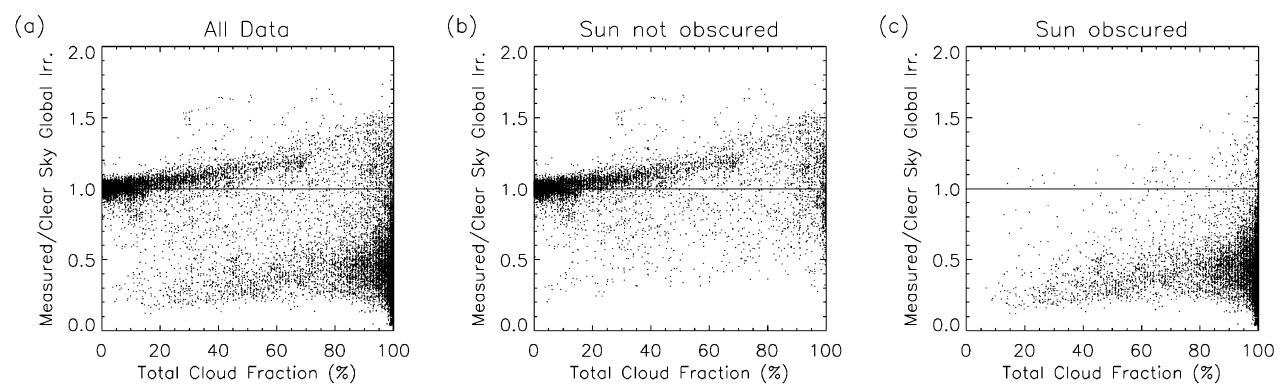
\includegraphics[width=\linewidth]{figures/misc/makoni_ietekme.jpg}
	\caption{Attiecība starp izmērīto apstarojumu un tīrās debess gadījuma apstarojumu (a) visiem datiem, (b) gadījumos ar neaizsegtu Sauli un (c) gadījumos ar aizsegtu Sauli~\cite{CloudCoverageImpactOnIrradiance}.}
	\label{fig:makoni_ietekme}
\end{figure}

Mākoņu ietekme ir atkarīga arī no to veida. Mākoņu modifikācijas reizinātājs (\textit{Cloud Modification Factor}, CMF), ko definē kā attiecību starp apstarojumu gadījumos ar un bez mākoņiem, atkarībā no mākoņu tipa ir apkopots \ref{tab:CMF}. tabulā. Ir jāņem vērā, ka CMF ir atkarīgs no viļņa garuma. Tomēr ultravioletais CMF no redzamās gaismas CMF ir atkarīgs lineāri ar koeficientiem $\approx0.6-1$ gubumākoņu gadījumā un eksponenciāli spalvmākoņu gadījumā~\cite{effectCloudsOnSurface}.

\begin{table}[h]
	\caption{CMF intervāls atkarībā no mākoņu tipa~\cite{effectCloudsOnSurface},~\cite{cloudAtlas}}
	\begin{center}
		\begin{tabular}{| r | c | c |}
			\hline
			Augstie gubumākoņi (\textit{Altocumulus}) & $<0.7$ & 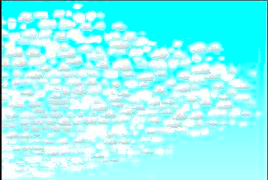
\includegraphics[width=0.1\linewidth]{figures/meteo/cloud_Altocumulus.jpg} \\ \hline
			Gubumākoņi (\textit{Cumulus})        & $0.2-1.3$ & 
\includegraphics[width=0.1\linewidth]{figures/meteo/cloud_Cumulus.jpg} \\ \hline
			Spalvmākoņi (\textit{Cirrus})        & $0.6-1$  & 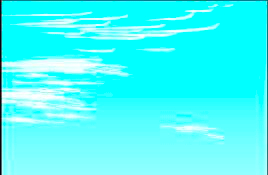
\includegraphics[width=0.1\linewidth]{figures/meteo/cloud_Cirrus.jpg} \\ \hline
		\end{tabular}
	\end{center}
	\label{tab:CMF}
\end{table}

Modelēt saules apstarojumu, kas nonāk paneļu virsmas, komplicē ne tikai mākoņu ietekme, bet arī Saules apstarojuma izmaiņas laikā. Tomēr šī darba ietvaros to var neņemt vērā, jo TSI mainās tikai ap $\pm 0.7$ W/m$^2$ gadā (solāro paneļu datu uzņemšanas laikā tas mainās par $\pm 0.225$ W/m$^2$ jeb 0.03 \%), kā tas ir redzams~\ref{fig:TSI2}. attēlā.

Atsaucoties uz TIM satelīta izmērīto saules gaismā ietverto enerģiju (skat.~\ref{fig:SSI}. att.), šis grafiks (skat.~\ref{fig:zudumi}. att.) attēlo enerģijas zudumus dažādiem viļņu garumiem absorbējoties atmosfērā, kā arī siltuma un sprieguma zudumus saules šūnā.

\begin{figure}[h]
    \centering
    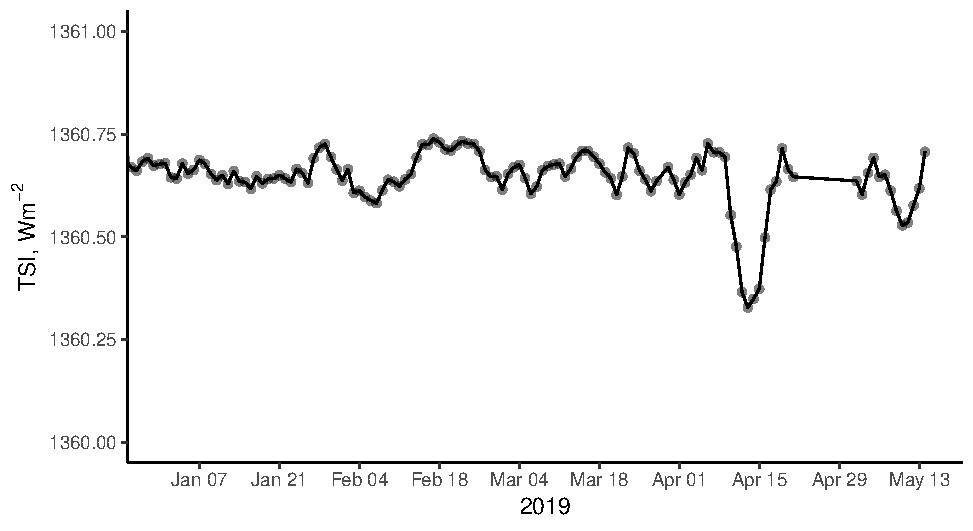
\includegraphics[width=\linewidth]{figures/misc/TSI.pdf}
    \caption{TSI izmaiņas solāro paneļu datu ieguves laikā 1 AU attālumā (24 h vidējā vērtība)\cite{TSIdata}.}
    \label{fig:TSI2}
\end{figure}


\begin{figure}[h]
    \centering
    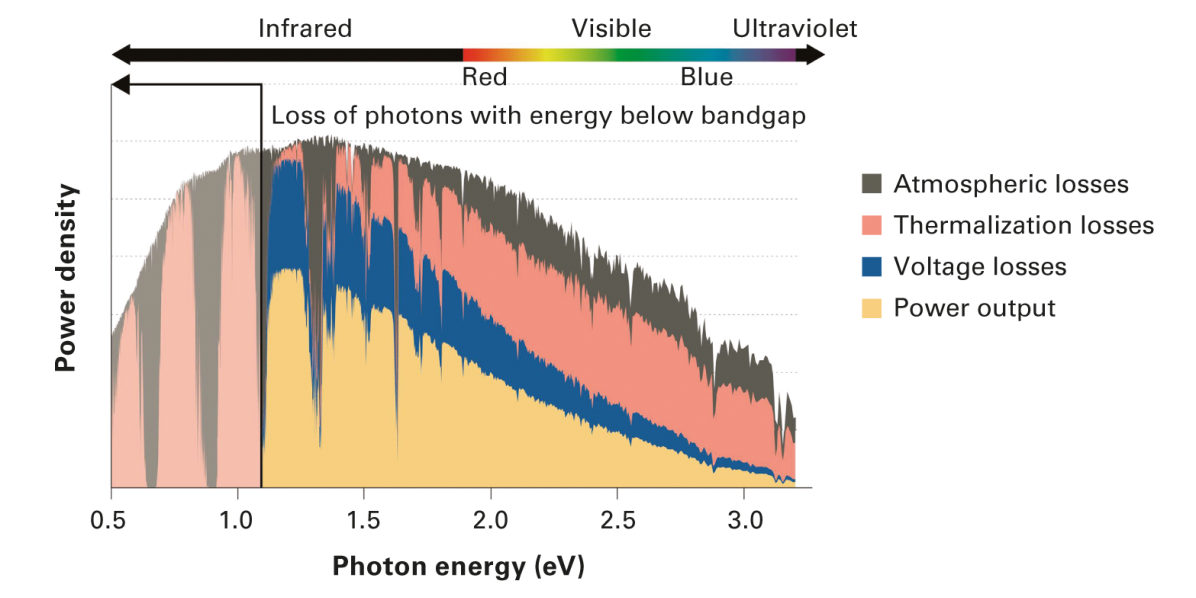
\includegraphics[width=\linewidth]{figures/misc/energyLosses.png}
    \caption{Saules enerģijas zudumi silīcijā balstītā saules šūnā.  ~\cite{Sivaram}.}
    \label{fig:zudumi}
\end{figure}

% DNI vidēji 1025 kWh/m2
% GHI vidēji arī bet vairāk

Pēc Solargis modeļa no satelītu un atmosfēras mērījumu datiem ar kļūdu 3\% līdz 10\% robežās secināms, ka piekrastē nonāk vairāk saules apstarojuma, tāpēc tur tiek prognozēta lielāka jauda~\ref{fig:lv_DNI}. Apstarojums iedalās vairākās kategorijās:
tiešais normālais apstarojums ir Saules apstarojums bez izkliedes atmosfērā.
Globālais horizontālais apstarojums (\textit{Global horizontal irradiance}, GHI) ir kopējais virsmas saņemtais apstarojums, ieskaitot gan DNI, gan starojumu, kas izkliedējas atmosfērā (\textit{Diffuse Horizontal Irradiance}, DHI). Šos lielumus savā starpā saista attiecība \ref{eq:YUCMWUH}~\cite{Sivaram}.

\begin{equation}
\label{eq:YUCMWUH}
\text{GHI}=\text{DHI} + \text{DNI}\times \cos(z)
\end{equation}

Salīdzinot \ref{fig:lv_GHI}. un  \ref{fig:lv_DNI}. attēlus redzams, ka GHI ir nedaudz lielāks par DNI, tātad redzams izkliedētā starojuma ieguldījums. Saules fotoelementa potenciālās jaudas (\textit{Photovoltaic power potential}, PVOUT) karte sniedz apkopojumu par prognozēto saules fotoelektrisko elementu (\textit{photovoltaics}, PV) enerģijas ražošanas apjomu, pieņemot 1kW jaudas Si materiāla PV spēkstacijas, gada patēriņam optimizētu slīpuma leņķi (skat. \ref{fig:lv_PVOUT}. att.). Pēc šiem datiem kopumā var secināt, ka saules paneļi ir piemērots risinājums enerģijas ieguvei arī Latvijā.

\begin{figure}[h]
    \centering
    \includegraphics[width=0.8\linewidth]{figures/misc/LV_DNI.png}
    \caption{Tiešais normālais apstarojums Latvijā \cite{solargis}}
    \label{fig:lv_DNI}
\end{figure}
\begin{figure}[h]
    \centering
    \includegraphics[width=0.8\linewidth]{figures/misc/LV_GHI.png}
    \caption{Globālais horizontālais apstarojums Latvijā \cite{solargis}}
    \label{fig:lv_GHI}
\end{figure}
\begin{figure}[t]
    \centering
    \includegraphics[width=0.8\linewidth]{figures/misc/LV_PVOUT.png}
    \caption{PV potenciālā jauda Latvijā \cite{solargis}}
    \label{fig:lv_PVOUT}
\end{figure}